%Analyzujte dostupná existující řešení BYOD, zejména z pohledu bezpečnosti.

Podle společnosti Gartner \todo{citace http://www.gartner.com/it-glossary/bring-your-own-device-byod/} je Bring your own device (BYOD) alternativní strategií pro povolení zaměstnancům, obchodním partnerům a dalším uživatelům používání osobně zvolených a pořízených koncových zařízení pro spouštění podnikových aplikací a přístup k datům.  Běžně zahrnuje chytré telefony a tablety, ale může být použita také pro osobní počítače. Může zahrnovat také dotaci od zaměstnavatele na pořízení zařízení.


Na problematiku nefiremních zařízení je možné nahlížet z různých pohledů. V této kapitole budou představeny různé možnosti dělení zařízení dle různých kategorií a taktéž budou představeny odpovídající řešení.

\todo{vice obecnych kecu o BYOD}

 \section{Různé pohledy na BYOD}
 \subsection{Rozdělení zařízení podle vlastnictví}
 Na základě vlastnictví zařízení je určena míra kontroly firmy zařízeními ve svojí síti.
 
 \subsubsection{Firemní zařízení}
 Jedná se o zařízení, které nakupuje a zároveň spravuje firma. Je ve vlastnictví firmy a pod dohledem IT oddělení. Zařízení plně splňuje politiky firmy a je plně kontrolované.
 
 \subsubsection{Externí firemní}
 Jedná se o firemní zařízení pracovníka externí firmy, jedná se tedy o firemní zařízení, ale o firemní zařízení jiné firmy. Je tedy pod správou IT oddělení externí firmy.
 
 Zařízení splňuje bezpečnostní politiky externí firmy a je kontrolované externí firmou. Není možné zařízení kontrolovat, je však možné vynutit potřebné bezpečnostní politiky smluvním vztahem s externí firmou.
 
 \subsubsection{Externí soukromé}
 Zařízení externího pracovníka, které není kontrolované firemní politikou externí firmy. Není možné jej kontrolovat a je obtížné vynucovat bezpečnostní politiky.
 
 \subsubsection{Zaměstnanec se soukromým zařízením}
 Vlastní zařízení zaměstnanců. Není kontrolované a může představovat bezpečnostní riziko.
 
 \subsection{Rozdělení podle typu zařízení}
 \subsubsection{PC}\todo{zdroj http://www.intel.com/content/www/us/en/tech-tips-and-tricks/pc-vs-mac-the-big-debate.html}
 V užším slova smyslu se jedná o osobní počítače s operačním systémem Windows od firmy Microsoft. Windows je aktuálně nejrozšířenější operační systém pro korporátní zařízení. Systém je určený pro zařízení postavené na architektuře x86. Typicky se jedná o stolní počítače a notebooky. Podle statistiky StatCounter\todo{zdroj: http://gs.statcounter.com/os-market-share/mobile-tablet/czech-republic/} měl operační systém Windows v únoru 2017 90 procentní podíl na trhu operačních systémů pro desktopy podle počtu přístupů na web. Podle celosvětových statistik přístupů na web v souhrnu všech typů zařízení podle StatCounter má však Windows pouze 38,6 procenta přístupů a je zřejmý trend mezi běžnými uživateli v upřednostňování jiných zařízení na úkor PC.\todo{zdroj: http://tech.ihned.cz/internet/c1-65653000-android-predbehne-windows-jako-nejpouzivanejsi-system-na-webu-v-cesku-mu-brani-draha-data}  
 
\begin{figure}[h]
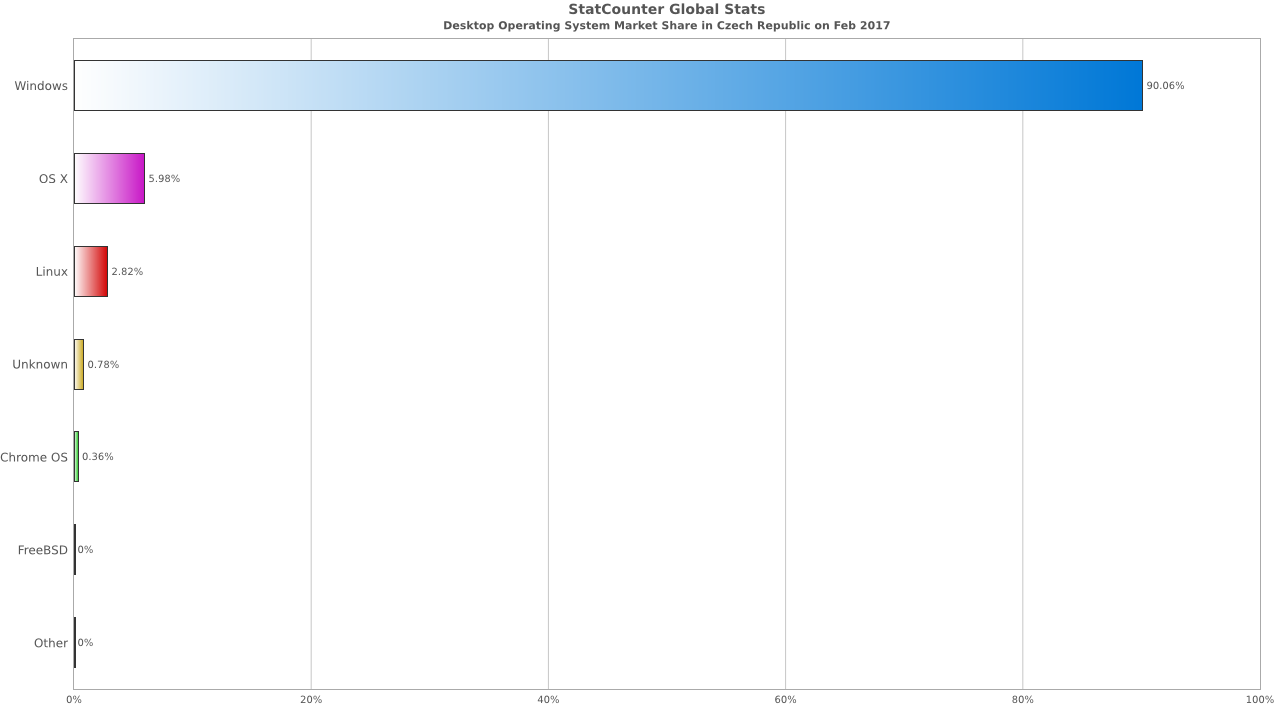
\includegraphics[width=13cm]{img/StatCounter_Desktop}
\caption{Statistika podílu operačních systémů pro desktopy v České republice podle přístupů na web. Převzato z \cite{http://gs.statcounter.com/os-market-share/mobile-tablet/czech-republic/}} 
\centering
\end{figure}\todo{citace}
 
 
 
 \subsubsection{Mac}\todo{zdroj http://www.apple.com/macos/what-is/}
 Počítač s operačním systémem MAC OS. Jedná se o proprietární operační systém pro počítače firmy Apple. Podle StatCounter je jeho podíl na trhu mezi desktopovými operačními systémy podle počtu přístupů na web v České republice necelých šest procent. Populární je zejména ve Spojených státech, kde se jeho podíl mezi desktopovými operačními systémy podle metodiky StatCounteru pohybuje okolo dvaceti procent.
 
 \begin{figure}[h]
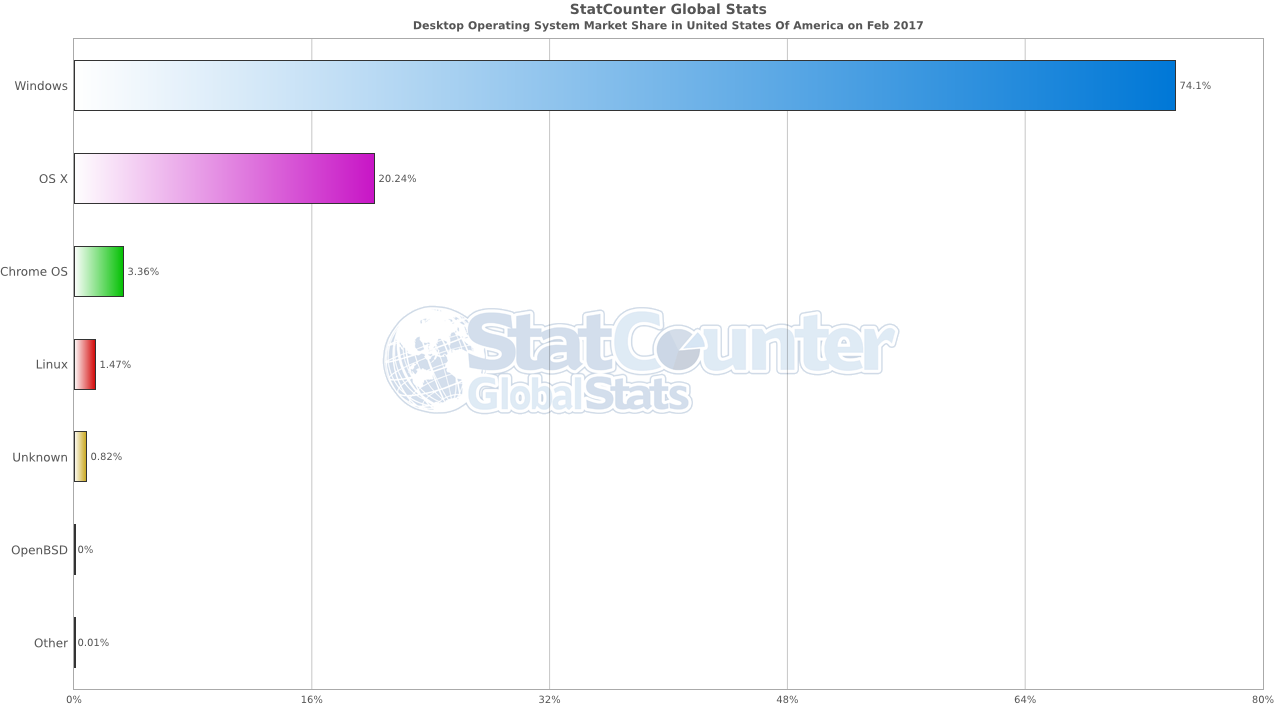
\includegraphics[width=13cm]{img/StatCounter_Destop_USA}
\caption{Statistika podílu operačních systémů pro desktopy v USA podle přístupů na web. Převzato z \cite{http://gs.statcounter.com/os-market-share/mobile-tablet/czech-republic/}} 
\centering
\end{figure}\todo{citace}
 
 
 \subsubsection{Chytrý telefon či tablet}
 Podle společnosti Gartner \todo{citace http://www.gartner.com/it-glossary/smartphone/} je chytrý telefon definován jako mobilní komunikační zařízení používající identifikovatelný otevřený operační systém. Tento systém je podporován aplikacemi třetích stran od komunity vývojářů. Aplikace třetích stran mohou být instalovány nebo odstraněny a mohou být vytvořeny přímo pro operační systém zařízení a aplikační programové rozhraní, případně pro oddělenou vrstvu jakou může být například Java. Operační systém musí podporovat multitaskingové prostředí a uživatelské rozhraní, které dokáže obsloužit více aplikací najednou. Například zobrazení emailu během přehrávání hudby.
 
 Obecněji se jedná mobilní zařízení s možností instalace aplikací. V současné době jsou nejpopulárnější zařízení s operačním systémem Android od firmy Google a iOS od firmy Apple. V České republice je podle metodiky měření společnosti StatCounter pro únor 2017 nejpopulárnější operační systém Android s podílem 68 procent. Operační systém iOS je na drůhém místě s podílem 26 procent. Více než jednoprocentní podíl má již pouze Windows s necelými čtyřmi procenty. \todo{citace http://tech.ihned.cz/internet/c1-65653000-android-predbehne-windows-jako-nejpouzivanejsi-system-na-webu-v-cesku-mu-brani-draha-data a statcounter}
 
 \begin{figure}[h]
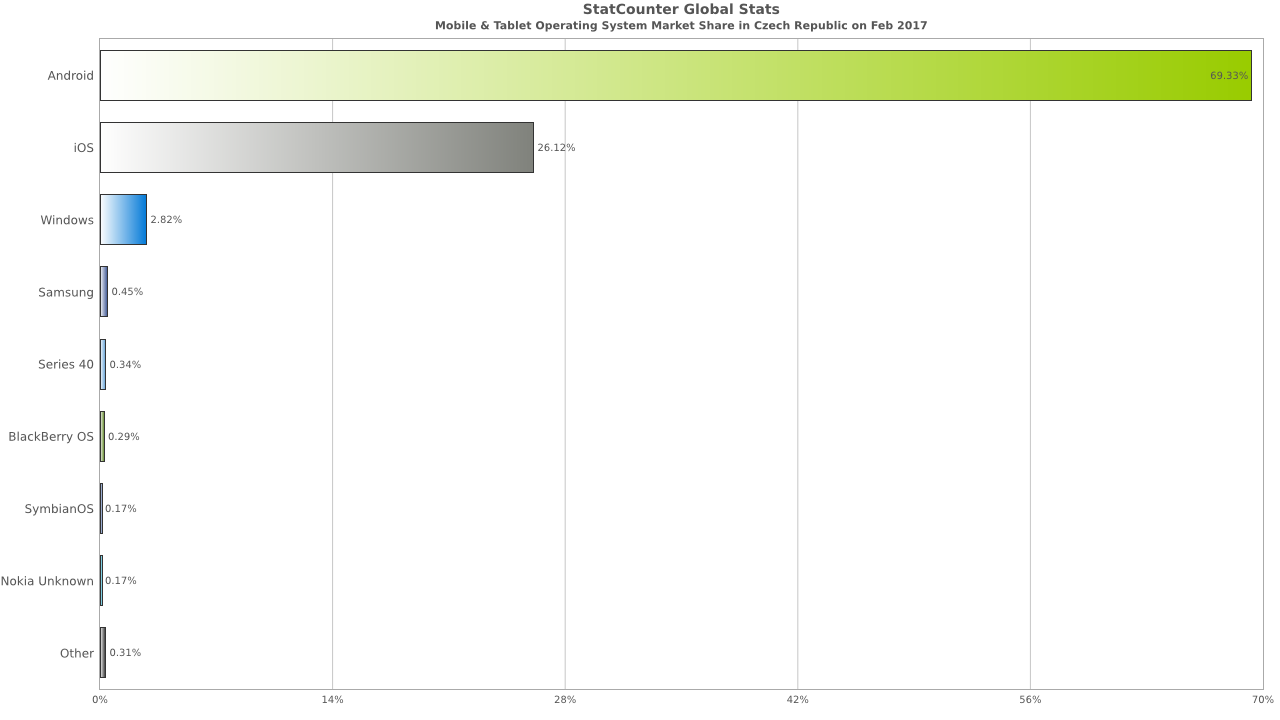
\includegraphics[width=13cm]{img/StatCounter_MobileBar}
\caption{Statistika podílu operačních systémů pro desktopy v České republice podle přístupů na web. Převzato z \cite{http://gs.statcounter.com/os-market-share/mobile-tablet/czech-republic/}} 
\centering
\end{figure}\todo{citace}
 
Celosvětově je zřejmá rostoucí obliba mobilních zařízení mezi uživateli a to především na úkor klasických PC s operačním systémem Windows. Vzhledem k postupné změně návyků uživatelů je třeba, aby firemní prostředí na tento trend vhodně reagovalo. 


\begin{figure}[h]
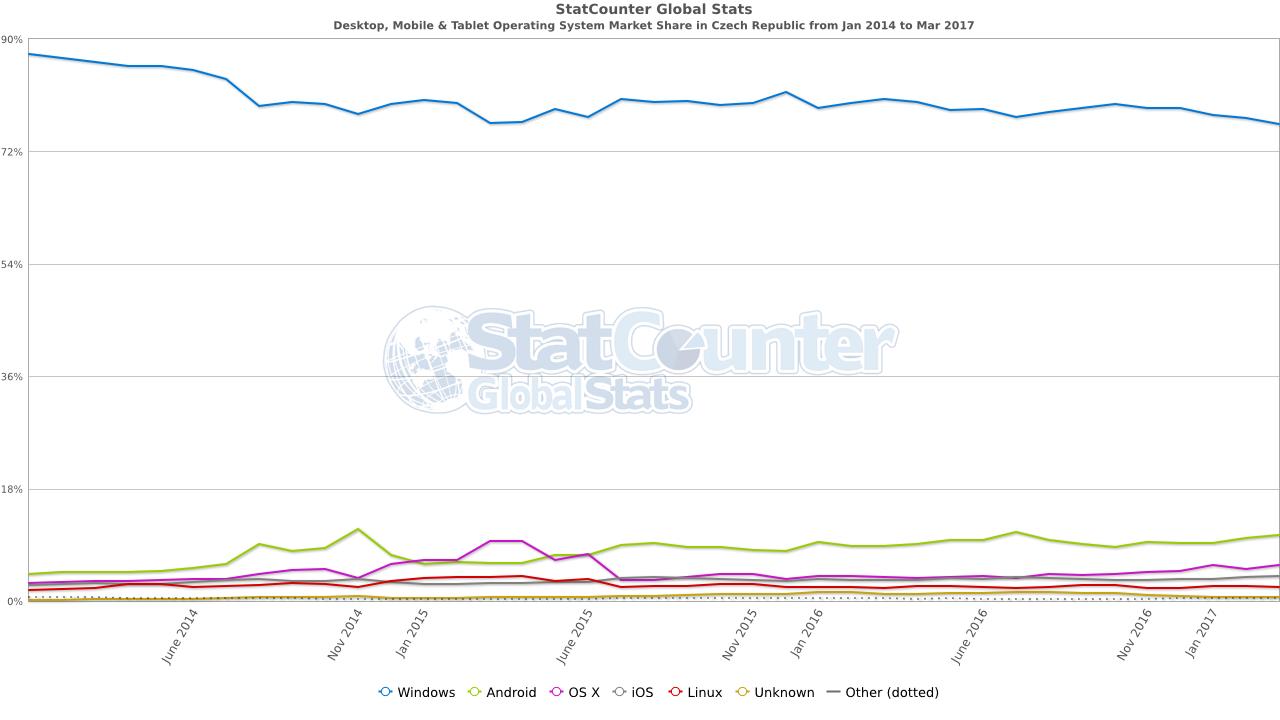
\includegraphics[width=13cm]{img/StatCounter_VyvojVse}
\caption{Statistika podílu všech operačních systémů pro desktopy v České republice podle přístupů na web. Převzato z \cite{http://gs.statcounter.com/os-market-share/mobile-tablet/czech-republic/}} 
\centering
\end{figure}\todo{citace}

\begin{figure}[h]
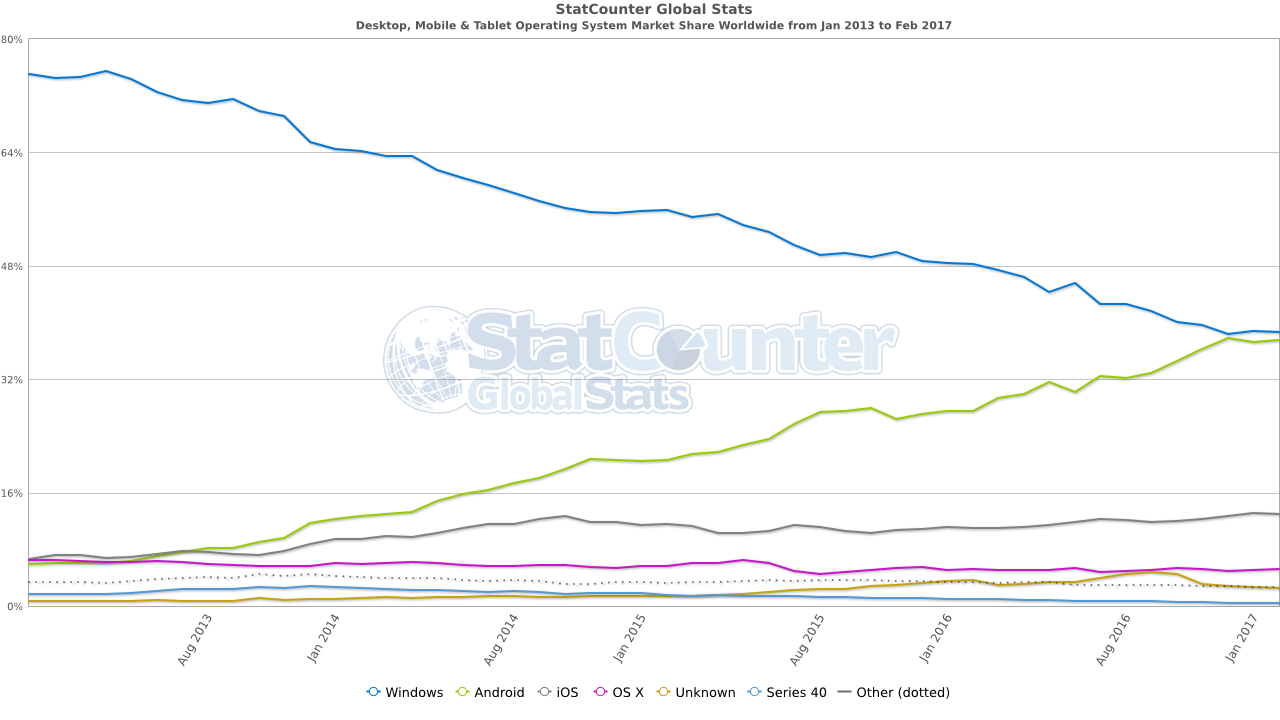
\includegraphics[width=13cm]{img/StatCounter_All_Worldwide}
\caption{Statistika podílu všech operačních systémů celosvětově podle přístupů na web. Převzato z \cite{http://gs.statcounter.com/os-market-share/}} 
\centering
\end{figure}\todo{citace}
 
Od těchto zařízení se nepředpokládá nutnost přístupu k podnikovým aplikacím, ale je vyžadován okamžitý přístup k emailům, kontaktům či dokumentům a to nezávisle na místě použití.

Report od společnosti Nokia Thread Intelligence Lab \todo{citovat http://resources.alcatel-lucent.com/asset/193174  http://www.nokia.com/en\_int/news/releases/2016/03/01/nokia-malware-report-shows-smartphones-now-account-for-60-of-infections-in-the-mobile-network}, který zmonitoroval aktivitu malware v sítích mobilních operátorů mezi lety 2012 a 2015 měly 60 \% veškeré aktivity malware v mobilních sítích na svědomí chytré telefony, zbytek šel na vrub Windows PC.

V prosinci 2015 vykazovalo známky napadení škodlivým software 0,3 \% všech chytých telefonů. Nejvíce napadení zaznamenali zařízení s operačním systémem Android, ovšem na seznam s dvaceti nejčastěji se vyskytujícími druhy školivého software so dostali i dva zástupci pro operašní systém iOS (XcodeGhost a Flexispy). V říjnu 2015 bylo 6 \% všech napadených zařízení značky iPhone.
 
 
 %%%%%%%%%%%%%%%%%%%%%%%%%%%%%%%%%%%%%%%%%%%%%%%%%%%%%%%%%%%%%%%%%%%%%%%%%%%%%%%%%%%%%%%%%%%%%%%%%%%%%%%%%%%%%%%%%%%%%%%%%%%%%%%%%%%
 \subsection{Rozdělení podle typu přístupu do datové sítě}
 \subsubsection{Ethernet}\todo{citace http://www.pcmag.com/encyclopedia/term/42781/ethernet}
 Jedná se o pevné připojení do korporátní sítě pomocí kabelu. Je vhodné pro firemní počítače, není vhodné pro zařízení typu mobilní telefon či tablet.
 
 Je definované ve standardu IEEE 802.3 \todo{Naflakat sem vic nesmyslu ze standardu}
 
 \subsubsection{Wi-Fi} \todo{http://www.pcmag.com/encyclopedia/term/54444/wi-fi}
 
 Bezdrátové připojení pomocí Wi-Fi sítí. Jedná se o standardní technologii pro bezdrátové sítě WLAN. Tento typ připojení je vhodný jak pro přenosné počítače, tak pro mobilní telefony či tablety.
 
 Wi-Fi je definovaná standardem IEEE 802.11
 
 \subsubsection{VPN} \todo{citace http://www.cisco.com/c/en/us/about/press/internet-protocol-journal/back-issues/table-contents-18/what-is-a-vpn.html}
 Virtual private network, čili vzdálené připojení do firemní sítě. Hlavním smyslem VPN je vytvořit soukromou síť pomocí tunelování a nebo šifrování skrze veřejný internet tak, aby uživatelé mohli vzdáleně přistupovat ke službám dostupným pouze zevnitř sítě.
 
 
 %%%%%%%%%%%%%%%%%%%%%%%%%%%%%%%%%%%%%%%%%%%%%%%%%%%%%%%%%%%%%%%%%%%%
 
 
 
 \section{Známé způsoby řešení BYOD}\todo{Zejmena z pohledu bezpecnosti}

\todo{doplnit typy hypervizoru/ typy virtualizace}
 
 \subsection{Centralizovaná virtualizace}
 Microsoft remote desktop, VMWare Horizon, Citrix XenDesktop
 \missingfigure{Magic quarter pro virtual dektopy}
 
 \todo{doplnit povidacky}
 
 \subsection{Distribuovaná virtualizace}
 Oracle Virtualbox, VMWare Fusion, VMWare Workstation, VMWare Fusion, VMWare Player, VMWare Horizon Flex
 
 \missingfigure{Taky nejaky hezky grafek}
 
 \subsection{DaaS}
 \todo{pouzit a citovat http://www.tomsitpro.com/articles/desktop-as-a-service-providers,2-838.html}
 Desktop as a service
 VMWare Horizon Air, Citrix XenDesktop, Amazon Work Spaces
 
 \todo{doplnit povidacky}
 
 \subsection{Rozlišení na úrovni sítě}
 Použitím Network Access Controll neboli NAC je možné spravovat přístup zařízení do sítě. Je možné nastavit autentifikační kontroly a další bezpečnostní politiky, které musí zařízení splňovat aby bylo do sítě vpuštěno. 
 
 Společnost Gartner identifikuje několik funkcí, které tato řešení nabízejí. \todo{citace https://www.gartner.com/doc/reprints?id=1-3I8W2V2\&ct=160922\&st=sb}
 Politiky mohou pojmout různé fukce jako například autentifikaci zařízení, autorizaci uživatele, lokaci, čas či přístup k aplikacím a zdrojům.
 
 Dále je možné posoudit stav zařízení z hlediska aktuálnosti systému a antivirových definic co se týče zařízení s Windows, nebo přítomnost EMM, viz \ref{EMM},  na mobilních zařízení.
 
 Přístup je přidělován pomocí síťové infrastruktury s použitím 802.1X protokolu, virtuálních LAN, či seznamů pro řízení přístupů neboli ACL (Access Control List).
 
 Dalšími službami poskytovanými NAC řešeními může být vytváření sítí pro hosty, monitoring připojených zařízení či integrace s dalšími bezpečnostními prvky.
 
 
Gartner ve své studii zmiňuje následující prudukty: Aruba ClearPass, Auconet BICS, Brandford Networks Network Sentry, Cisco ISE, Extreme Networks ExtremeControll, ForeScout CounterACT, Impulse Point SafeConnect, Info Express CGX, Portnox CLEAR, Pulse Policy Secure, SnoopWall Netshield.
 
 
 \subsubsection{Virtualizace aplikaci}
 Další možností je nevirtualizovat celý operační systém, ale pouze aplikace. Mezi výhody patří snadná aktualizace aplikací, snadná správa přístupu k aplikacím či nenáročnost na výpočetní výkon klienta.
 
 Mezi hlavní nevýhody patří problémy s periferiemi jako např. tiskárny či nutnost stálé a kvalitní konektivity.
 
  Nejznámějšími poskytovateli virtualizace aplikací jsou Citrix XenApp, Citrix XenDesktop, VMware Horizon, Dell vWorkspace, and Microsoft RDSH\todo{překlad}
 
 
 \subsubsection{EMM/EMS}\label{EMM}
 Enterprise mobility management nebo též Enterprise Mobility suite umožňují integrovat a spravovat mobilní zařízení v rámci firemní infrastruktury.
 Dle agentury Gartner jsou EMM balíky lepidlem, které připojuje mobilní zařízení do firemní infrastruktury. \cite{Gartner_EMM_2016}
 
 EMM mají následující funkce:
 \begin{itemize}
     \item nastavují zařízení a aplikace pro nasazení ve firemním prostředí
     \item sledují dodržení firemních politik a spravují firemní aktiva
     \item snižují riziko ztráty dat, krádeže či dalších incidentů řízením šifrování dat, přístupových práv, sdílených zařízení, obalování aplikací či zamknutí zařízení.
     \item umožňují vzdálenou podporu zařízení pro IT oddělení
 \end{itemize}
 
Výzkum společnosti J Gold Associates z roku 2016 \todo{citace http://jgoldassociates.com/Technology\_Brief/Technology\_Brief\_April\_2016.pdf} ukazuje, že firmy v drtivé většině nenasazují všechny funkce, které EMM řešení nabízejí. Nejpoužívanější funkce EMM jsou vypsány na obrázku (\ref{funkceEMM}) 

\begin{figure}[h!]
\centering
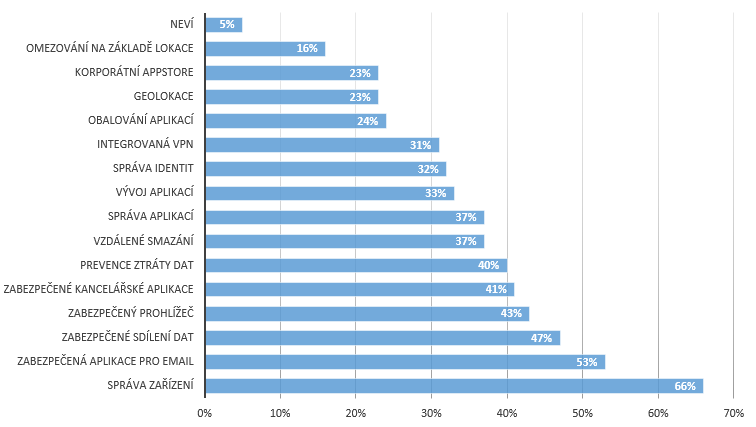
\includegraphics[width=13cm]{img/funkceEMM}
\caption{Které komponenty EMM řešení organizace zapojené do průzkumu aktuáně používají? } 
\end{figure}\label{funkceEMM}
\todo{citace http://jgoldassociates.com/Technology\_Brief/Technology\_Brief\_April\_2016.pdf}
 
 
 
  \subsection{MDM}
 Mobile device management je software pro správu mobilního zařízení. Je podmnožinou EMM. Mezi základní funkce tohoto software patří podle \todo{citace: FEL BYOD vosykto} patří:
 \begin{itemize}
     \item Automatické nastavení mobilního zařízení. Umožňuje IT oddělení nastavit zařízení podle firemních potřeb. To zahrnuje instalaci bezpečnostních certifikátů, nastavení uživatelských účtů či dalších nastavení umožňující přístup k firemní síti.
     \item Možnost vzdáleného vymazání. Umožňuje vzdáleně vymazat data tak, aby nebyly dostupné. To je užitečné v případě ztráty či krádeže zařízení, nebo po ukončení pracovního poměru se zaměstnancem.
     \item Vynucení bezpečnostních politik. To zahrnuje vynucení silného hesla, šifrování dat či omezení některých funkcí jako je například propojení se soukromým cloudovým úložištěm. 
     \item Detekce jailbreak/root zařízení. Detekuje spuštění zařízení v administrátorském režimu, což je ve firemním prostředí nepřípustné.
     \item Blacklisting/whitelisting aplikací. Umožňuje správci zařízení zvolit, které aplikace je a není možné instalovat.
     \item Monitoring. Umožňuje sledovat přistupování uživatele k jednotlivým službám.
     \item Administrace. Umožňuje hromadné aktualizace, instalace či odinstalace aplikací pro zařízení ve firemní flotile.
 \end{itemize}
 
 %MobileIron, VMWare Air Watch \ldots 
 %\missingfigure{Magic quarter pro MDM}
 
 \subsection{MAM} 
 Mobile application management. MAM je též podmnožinou EMM. Narozdíl od MDM nespravuje zařízení jako celek, ale pouze podnikové aplikace. Tyto aplikace jsou získávány přes speciální obchod s aplikacemi. Mezi hlavní funkce MAM patří:
 \begin{itemize}
     \item Podnikový obchod s aplikacemi. Umožňuje nasazování jak vlastních tak komerčních aplikací pro potřeby businessu.
     \item Podporu pro správu a distribuci aplikací s užitím API operačního systému či hromadného nákupu aplikací.
     \item Kontejnerizace aplikací
     \item Reporting o užívání aplikací
 \end{itemize}
 
 Podle \cite{Gartner_EMM_2016} jsou pomocí MAM běžně uplatňovány následující politiky:
 \begin{itemize}
     \item Vyžadování iniciace VPN spojení pro aplikaci při spuštění
     \item Šifrování podnikových dat (často s použitím silnějšího šifrování než by bylo použito v rámci operačního systému)
     \item Omezení sdílení dat mezi aplikacemi pouze na podnikové aplikace
     \item Omezení copy/paste funkcionality
     \item Vyžadování specifického stavu při spuštění nebo při přístupu -- například nebyl detekován root nebo jailbreak
 \end{itemize}
 
  
\begin{figure}[h]
\centering
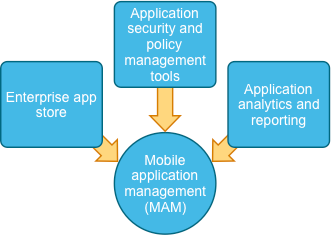
\includegraphics[width=7cm]{img/MAM-Offering}
\caption{Gartner Magic quadrant. Převzato z } 
\label{MAM:nacrt}
\end{figure}\todo{ citace https://www.ibm.com/developerworks/community/blogs/mobileblog/entry/got\_mam\_mobile\_application\_management\_in\_your\_2013\_mobile\_menu25?lang=en}


\subsection{MCM} 
Mobile content management. Jedná se o software pro správu obsahu na mobilních zařízeních. podle \cite{Gartner_EMM_2016} má tři základní role:
\begin{itemize}
    \item Vynucování politik Dokáže vynutit politiky pro jednotlivé soubory včetně šifrovacích klíčů nezávislých na zařízení, autentifikace, pravidel pro sdílení souborů či pravidel pro copy and paste funkcionalitu.
    \item Přístup k obsahu. Vynutí pravidla pro distribuci, záměnu a mazání souborů.
    \item Integrace Přidává kompaktibilitu pro systémy správy práv, jako jsou ochrana ztráty dat (DLP) nebo podniková správa práv (EDRM) od třetích stran.
\end{itemize}
 
